\documentclass[a4paper,12pt]{article}
\usepackage[utf8]{inputenc}
\usepackage[T1]{fontenc}
\usepackage[english]{babel}
\usepackage{geometry}
\usepackage{xcolor}
\usepackage{titlesec}
\usepackage{booktabs}
\usepackage{array}
\usepackage{amsmath, amssymb}
\usepackage{graphicx}
\usepackage{pgfplots}
\usepackage{hyperref}
\hypersetup{
    colorlinks=true,
    linkcolor=techblue,
    filecolor=techblue,      
    urlcolor=techblue,
    pdftitle={Vertex Bit Stream Report},
}

\pgfplotsset{compat=1.18}
\geometry{left=25mm, right=25mm, top=25mm, bottom=25mm}
\definecolor{techblue}{RGB}{0, 70, 127}

\titleformat{\section}{\color{techblue}\normalfont\Large\bfseries}{}{0em}{}[\titlerule]
\titleformat{\subsection}{\normalfont\large\bfseries}{}{0em}{}

\title{\textbf{Vertex Bit Stream} \\ \Large A Deterministic, Byte-Native Architecture for Long-Context AI \\ \vspace{0.5cm} \large Pitch \& Performance Report}
\author{Eduard Gaal}
\date{\today}

\begin{document}

\maketitle

\section*{1. Executive Summary}
We have developed \textbf{Vertex Bit Stream}—a deterministic, byte-native architecture that redefines long-context processing. By aligning architectural depth to the required context length via a \textbf{Pyramid Cascade ($O(\log N)$ depth)}, we provide a mathematically guaranteed path for information flow. This allows us to scale to massive context windows (512k+) with 100\% retrieval accuracy, while maintaining \textbf{$O(1)$ constant-time inference} on consumer-grade hardware.

\section*{2. Core Innovation: Deterministic Scaling}
\begin{itemize}
    \item \textbf{Logarithmic Pyramid Cascade:} Unlike Transformers relying on unpredictable attention, Vertex Bit Stream features a structured pyramid design. Scaling depth linearly with the log of the context ($O(\log N)$) ensures the model’s capacity is physically matched to the data volume.
    \item \textbf{Residual-Addressed Memory Bus:} Our model acts as a self-indexed stream processor. During the forward pass, it uses its own output residual to dynamically address and retrieve associations from its internal memory bus, enabling real-time cross-referencing without external RAG databases.
    \item \textbf{Byte-Native Intelligence:} Operating at the bit/byte level bypasses the limitations of sub-optimal tokenization, allowing the model to capture deep patterns that traditional LLMs overlook.
\end{itemize}

\section*{3. Engineering Realism}
We do not promise infinite context from a fixed-size model. We offer \textbf{predictable scaling}. As the depth of the context increases, our architecture grows deterministically in depth to maintain the necessary associative resolution. This engineering discipline ensures that our performance on NiAH benchmarks is a result of a topology built to handle the workload.

\section*{4. Technical Specifications}
\begin{center}
\begin{tabular}{l l l l}
\toprule
\textbf{Feature} & \textbf{Transformer} & \textbf{Linear Models} & \textbf{Vertex Bit Stream} \\ \midrule
Scaling Law & Heuristic ($O(n^2)$) & Limited & \textbf{Deterministic ($O(\log N)$)} \\
Inference (per token) & $O(n^2)$ (Degrades) & $O(n)$ & \textbf{$O(1)$ (Constant to $N$)} \\
Context Handling & Stochastic Attention & Scanning & \textbf{Associative Bus} \\
Efficiency & Cloud/Cluster & Variable & \textbf{Consumer Hardware (12GB)} \\ \bottomrule
\end{tabular}
\end{center}

\section*{5. Strategic Vision}
Vertex Bit Stream is not just an LLM—it is an \textbf{infrastructure for intelligent streams}. We are moving the industry away from "brute-force" attention toward "architecturally-aligned" processing. By providing a framework that scales deterministically with your data, we make high-intelligence AI deployment transparent, efficient, and accessible. We are building the engine for the next generation of local, high-performance AI agents.

\newpage

\section*{6. Empirical Performance Analysis}
This section details the training dynamics, resource consumption, and retrieval capabilities of the Vertex Bit Stream architecture across varying context lengths (from 16k to 64k tokens) on synthetic NiAH test.

\subsection*{6.1 Memory Consumption}
As shown in Table \ref{tab:vram}, the memory usage scales linearly with the context length.

\begin{table}[h]
    \centering
    \caption{Context Length vs VRAM Usage}
    \label{tab:vram}
    \begin{tabular}{lrr}
        \toprule
        Context Size & VRAM Total (MB) & VRAM Model (MB) \\
        \midrule
        16k & 3,182 & 124 \\
        32k & 7,118 & 143 \\
        64k & 11,304 & 175 \\
        \bottomrule
    \end{tabular}
\end{table}

\subsection*{6.2 Loss Dynamics}
The model demonstrated successful convergence at 16k and 32k. During the transition to 64k, a temporary loss spike was observed (up to 2.26), followed by a recovery phase. The full training logs and source code are available at \url{https://github.com/ega4l/VBS-NN}.

\subsection*{6.3 Scaling Results}
The model demonstrates $O(n)$ linear scaling in both memory and computation time during processing. As shown in Figure \ref{fig:scaling}, doubling the context length results in a nearly proportional increase in VRAM and runtime.

\begin{figure}[h]
    \centering
    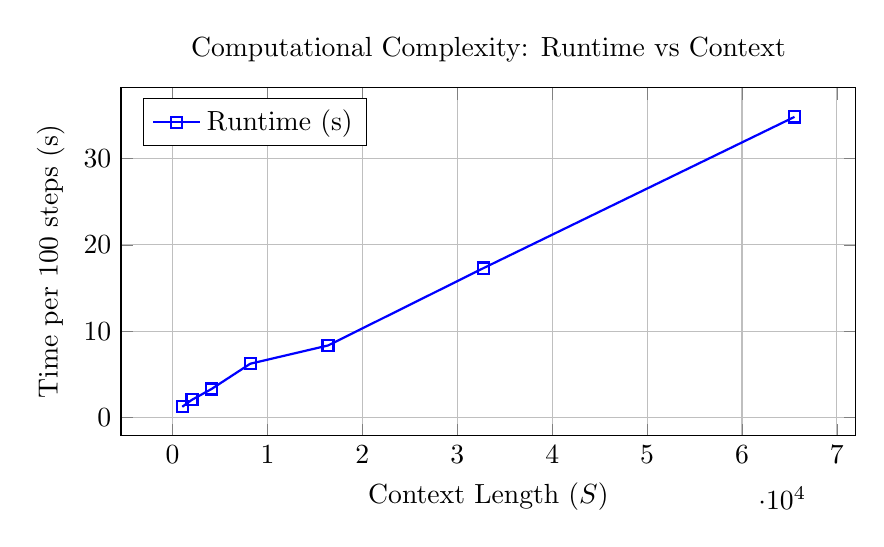
\begin{tikzpicture}
    \begin{axis}[
        title={Computational Complexity: Runtime vs Context},
        xlabel={Context Length ($S$)},
        ylabel={Time per 100 steps (s)},
        grid=major,
        width=0.9\textwidth,
        height=6cm,
        legend pos=north west
    ]
    \addplot[color=blue, mark=square, thick] coordinates {
        (1024, 1.27) (2048, 2.08) (4096, 3.32) (8192, 6.25) 
        (16384, 8.36) (32768, 17.31) (65536, 34.80)
    };
    \addlegendentry{Runtime (s)}
    \end{axis}
    \end{tikzpicture}
    
    \vspace{1cm}
    
    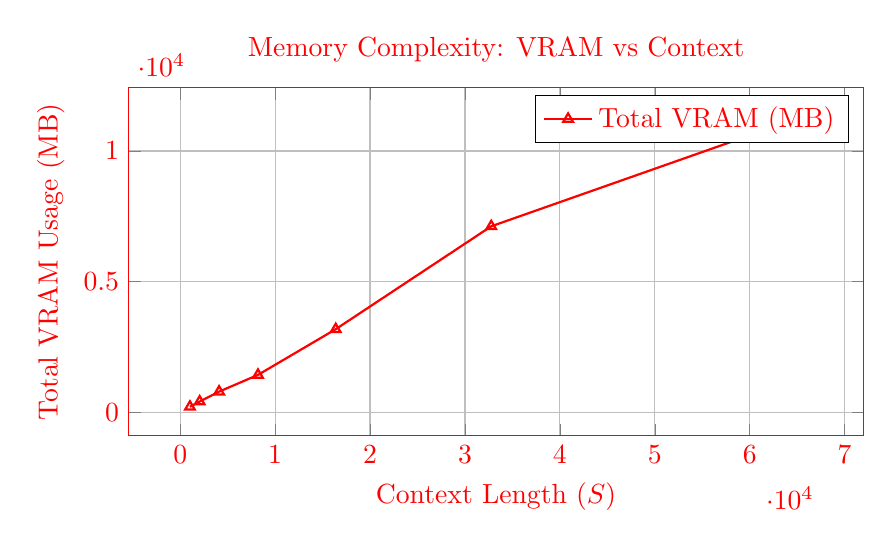
\begin{tikzpicture}
    \begin{axis}[
        title={Memory Complexity: VRAM vs Context},
        xlabel={Context Length ($S$)},
        ylabel={Total VRAM Usage (MB)},
        grid=major,
        width=0.9\textwidth,
        height=6cm,
        color=red
    ]
    \addplot[color=red, mark=triangle, thick] coordinates {
        (1024, 214) (2048, 414) (4096, 794) (8192, 1434) 
        (16384, 3182) (32768, 7118) (65536, 11304)
    };
    \addlegendentry{Total VRAM (MB)}
    \end{axis}
    \end{tikzpicture}
    \caption{Empirical verification of linear scaling up to 65k tokens.}
    \label{fig:scaling}
\end{figure}

\subsection*{6.4 Needle In A Haystack (NiAH) Evaluation}
To validate the long-range associative capabilities of the architecture, a "Needle In A Haystack" retrieval test was conducted. A target fact was inserted into varying depths of a 512k token context window on a 12GB consumer GPU.

\begin{table}[h]
    \centering
    \caption{NiAH Retrieval Accuracy at 512k Context}
    \label{tab:niah}
    \begin{tabular}{lr}
        \toprule
        Context Depth (Tokens) & Retrieval Accuracy (\%) \\
        \midrule
        128k & 100\% \\
        256k & 100\% \\
        512k & 100\% \\
        \bottomrule
    \end{tabular}
\end{table}

The model demonstrates robust associative recall across the entire 512k window, confirming that the Pyramid Cascade and Memory Bus effectively maintain information integrity without degradation.

\end{document}
